\begin{figure}[h!]
	\centering
	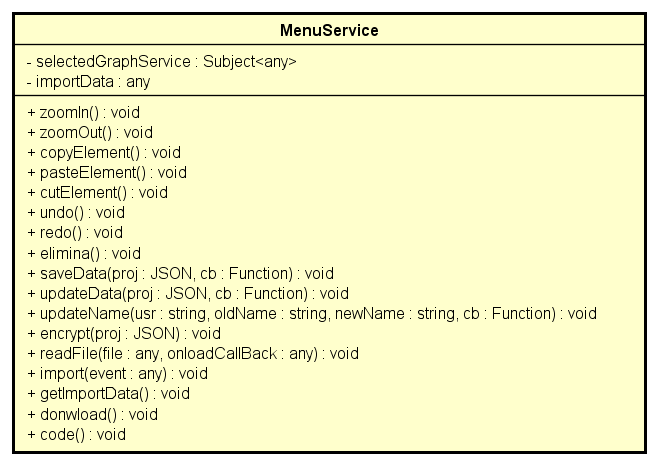
\includegraphics[scale=0.8]{res/sections/SpecificaFrontEnd/Services/Disegnetti/menu.png}
	\caption{Diagramma della classe MenuService}
\end{figure}

\begin{itemize}
	\item \textbf{Descrizione:}\\
	
	\item \textbf{Utilizzo:}\\
	
	\item \textbf{Attributi:}
		\begin{itemize}
			\item \emph{-selectedGraphService: Subject<any>}\\
			Memorizza l'array con tutte le shape
			\item \emph{-importData: any}\\
			Serve per importare il progetto
		\end{itemize}
	\item \textbf{Metodi:}
		\begin{itemize}
			\item \emph{+zoomIn()}\\
    		Esegue lo zoom in avanti
    		\item \emph{+zoomOut()}\\
    		Esegue lo zoom all'indietro
    		\item \emph{+copyElement()}\\
    		Copia l'elemento selezionato
    		\item \emph{+pasteElement()}\\
    		Incolla l'elemento copiato/tagliato
    		\item \emph{+cutElement()}\\
    		Taglia l'elemento selezionato
    		\item \emph{+undo()}\\
    		Annulla l'ultima operazione
    		\item \emph{+redo()}\\
    		Ripristina l'azione annullata
    		\item \emph{+elimina()}\\
    		Elimina l'elemento selezionato
    		\item \emph{+saveData(proj: JSON, cb: Function)}\\
    		Richiede al server dei dati del progetto corrente memorizzati nel database\\
    		\textbf{Parametri:}
    		\begin{itemize}
    			\item \emph{proj: JSON}\\
    			Progetto corrente
    			\item \emph{cb: Function}\\
    			Funzione
    		\end{itemize}
    		\item \emph{+updateData(proj: JSON, cb: Function)}\\
    		Aggiorna i dati del progetto corrente nel database\\
    		\textbf{Parametri:}
    		\begin{itemize}
    			\item \emph{proj: JSON}\\
    			Progetto corrente
    			\item \emph{cb: Function}\\
    			Funzione
    		\end{itemize}
    		\item \emph{+updateName(usr: string, oldName: string, newName: string, cb: Function)}\\
    		Aggiorna il nome del progetto corrente\\
    		\textbf{Parametri:}
    		\begin{itemize}
    			\item \emph{usr: string}\\
    			Nome utente
    			\item \emph{oldName: string}\\
    			Vecchio nome del progetto
    			\item \emph{newName: string}\\
    			Nuovo nome del progetto
    			\item \emph{cb: Function}\\
    			Funzione
    		\end{itemize}
    		\item \emph{+encrypt(proj: JSON)}\\
    		Richiede al server la funzione di criptazione\\
    		\textbf{Parametri:}
    		\begin{itemize}
    			\item \emph{proj: JSON}\\
    			Progetto da criptare
    		\end{itemize}
    		\item \emph{+readFile(file: any, onloadCallBack: any)}\\
    		Legge un file esterno\\
    		\textbf{Parametri:}
    		\begin{itemize}
    			\item \emph{file: any}\\
    			File da caricare
    			\item \emph{onloadCallBack: any}\\
    			Funzione
    		\end{itemize}
    		\item \emph{+import(event: any)}\\
    		Importa un file esterno\\
    		\textbf{Parametri:}
    		\begin{itemize}
    			\item \emph{event: any}\\
    			File da importare
    		\end{itemize}
    		\item \emph{+getImportData()}\\
    		Ritorna importData
    		\item \emph{+donwload()}\\
    		Richiede al server la funzione di parsing e download
    		\item \emph{+code()}\\
    		Richiama la funziona di download
		\end{itemize}
\end{itemize}